\chapter{系统总体组成与核心机制}

\mbox{BioMed QAgent} 的整体设计遵循一个核心原则：开放式理解交给LLM，正式数据操作交给确定性Dataset Core。两者通过声明式规格与事件日志衔接，因此“找到什么、如何解析、怎样清洗、来自哪里、输出为何种形式”都可以检查和回溯。主图给出整体分层及其与赛题评分维度的对应关系——即数据查找完备性、来源可追溯性、清洗整合可靠性与输出格式可用性四项。本章介绍Core 之外的部分；Dataset Core 内部的固定流水线在第四章展开。

\begin{figure}[htbp]
\centering
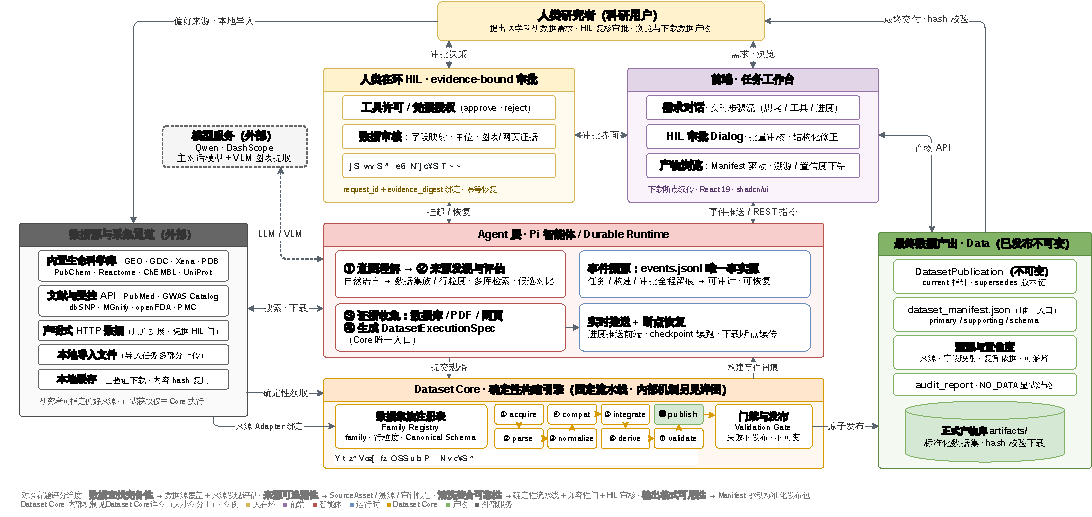
\includegraphics[width=1.00\textwidth]{figures/biomed-qagent-main.pdf}
\caption{\mbox{BioMed QAgent} 主架构。正式写入由 Core 检查；人工验收的请求处理与实际触发情况分别见\ref{sec:hil} 节、\ref{sec:corrected-six-run} 节。}\label{fig:main-architecture}
\end{figure}

\section{系统组成总览}

Dataset Core 负责正式数据处理与发布。其余五部分负责交互、模型调用、任务运行、来源访问和人工确认：

\begin{itemize}
  \item 前端任务工作台：提供需求对话、工具进度、人工确认和发布物浏览。研究者可以查看来源记录、处理过程、检查结果，并下载清单列出的文件（图~\ref{fig:ui-workbench}）。
  \item 模型服务：通过 DashScope 等接口调用 Qwen 主对话模型和视觉模型。模型提出查询、字段映射或变换代码；生成候选文件不等于获得正式发布权。
  \item Agent 层：理解需求、发现来源、收集证据，并向 Core 提交数据集执行规格。运行事件用于记录进度和恢复任务。
  \item 数据源与采集通道：包括 GEO、GDC、Xena、PDB、PubChem、Reactome、ChEMBL、UniProt 等数据库，文献及受控 API，声明式 HTTP 数据源、本地导入与缓存。正式输入需由 Core 获取或登记为任务来源资产。
  \item 人工确认（Human-in-the-Loop，HIL）：处理许可、数据审核与发布验收。审批类型可采用人工审核、模型初审或自动通过；其中要求人工处理的请求不接受模型代审。具体规则见\ref{sec:hil} 节。
\end{itemize}

\begin{figure}[htbp]
\centering
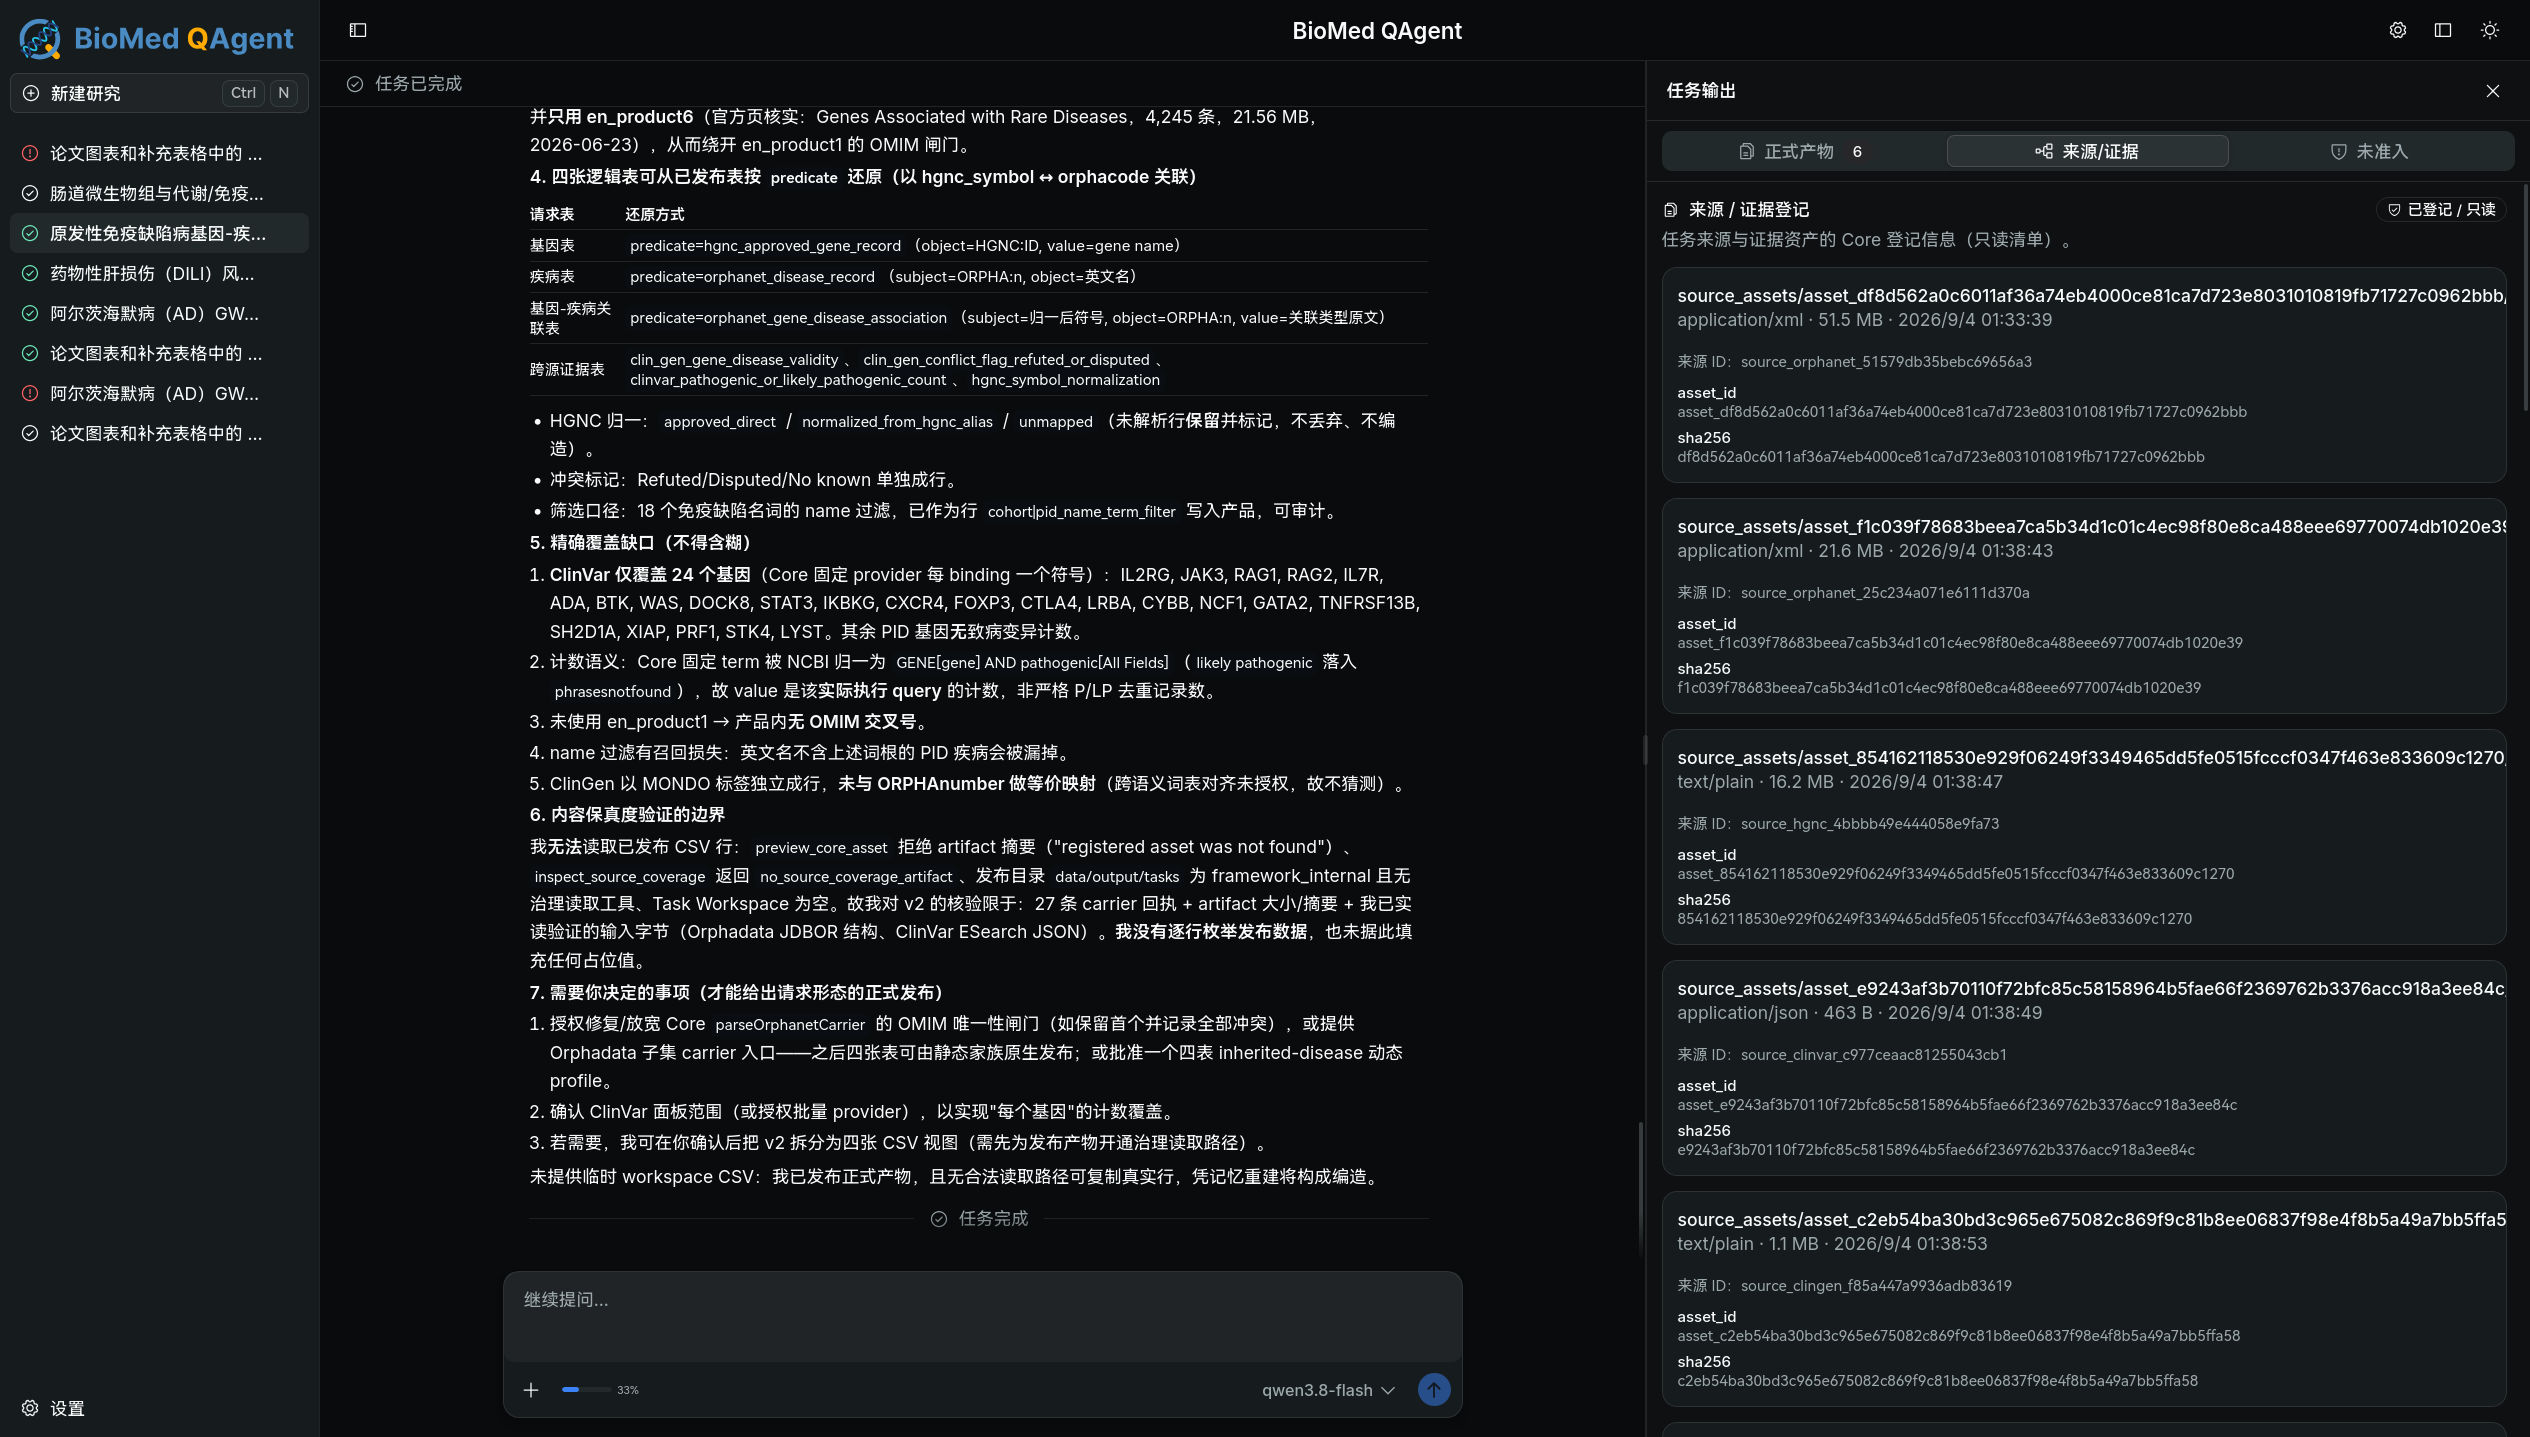
\includegraphics[width=0.90\textwidth]{figures/ui-gold9-source-registry.png}\\[0.4em]
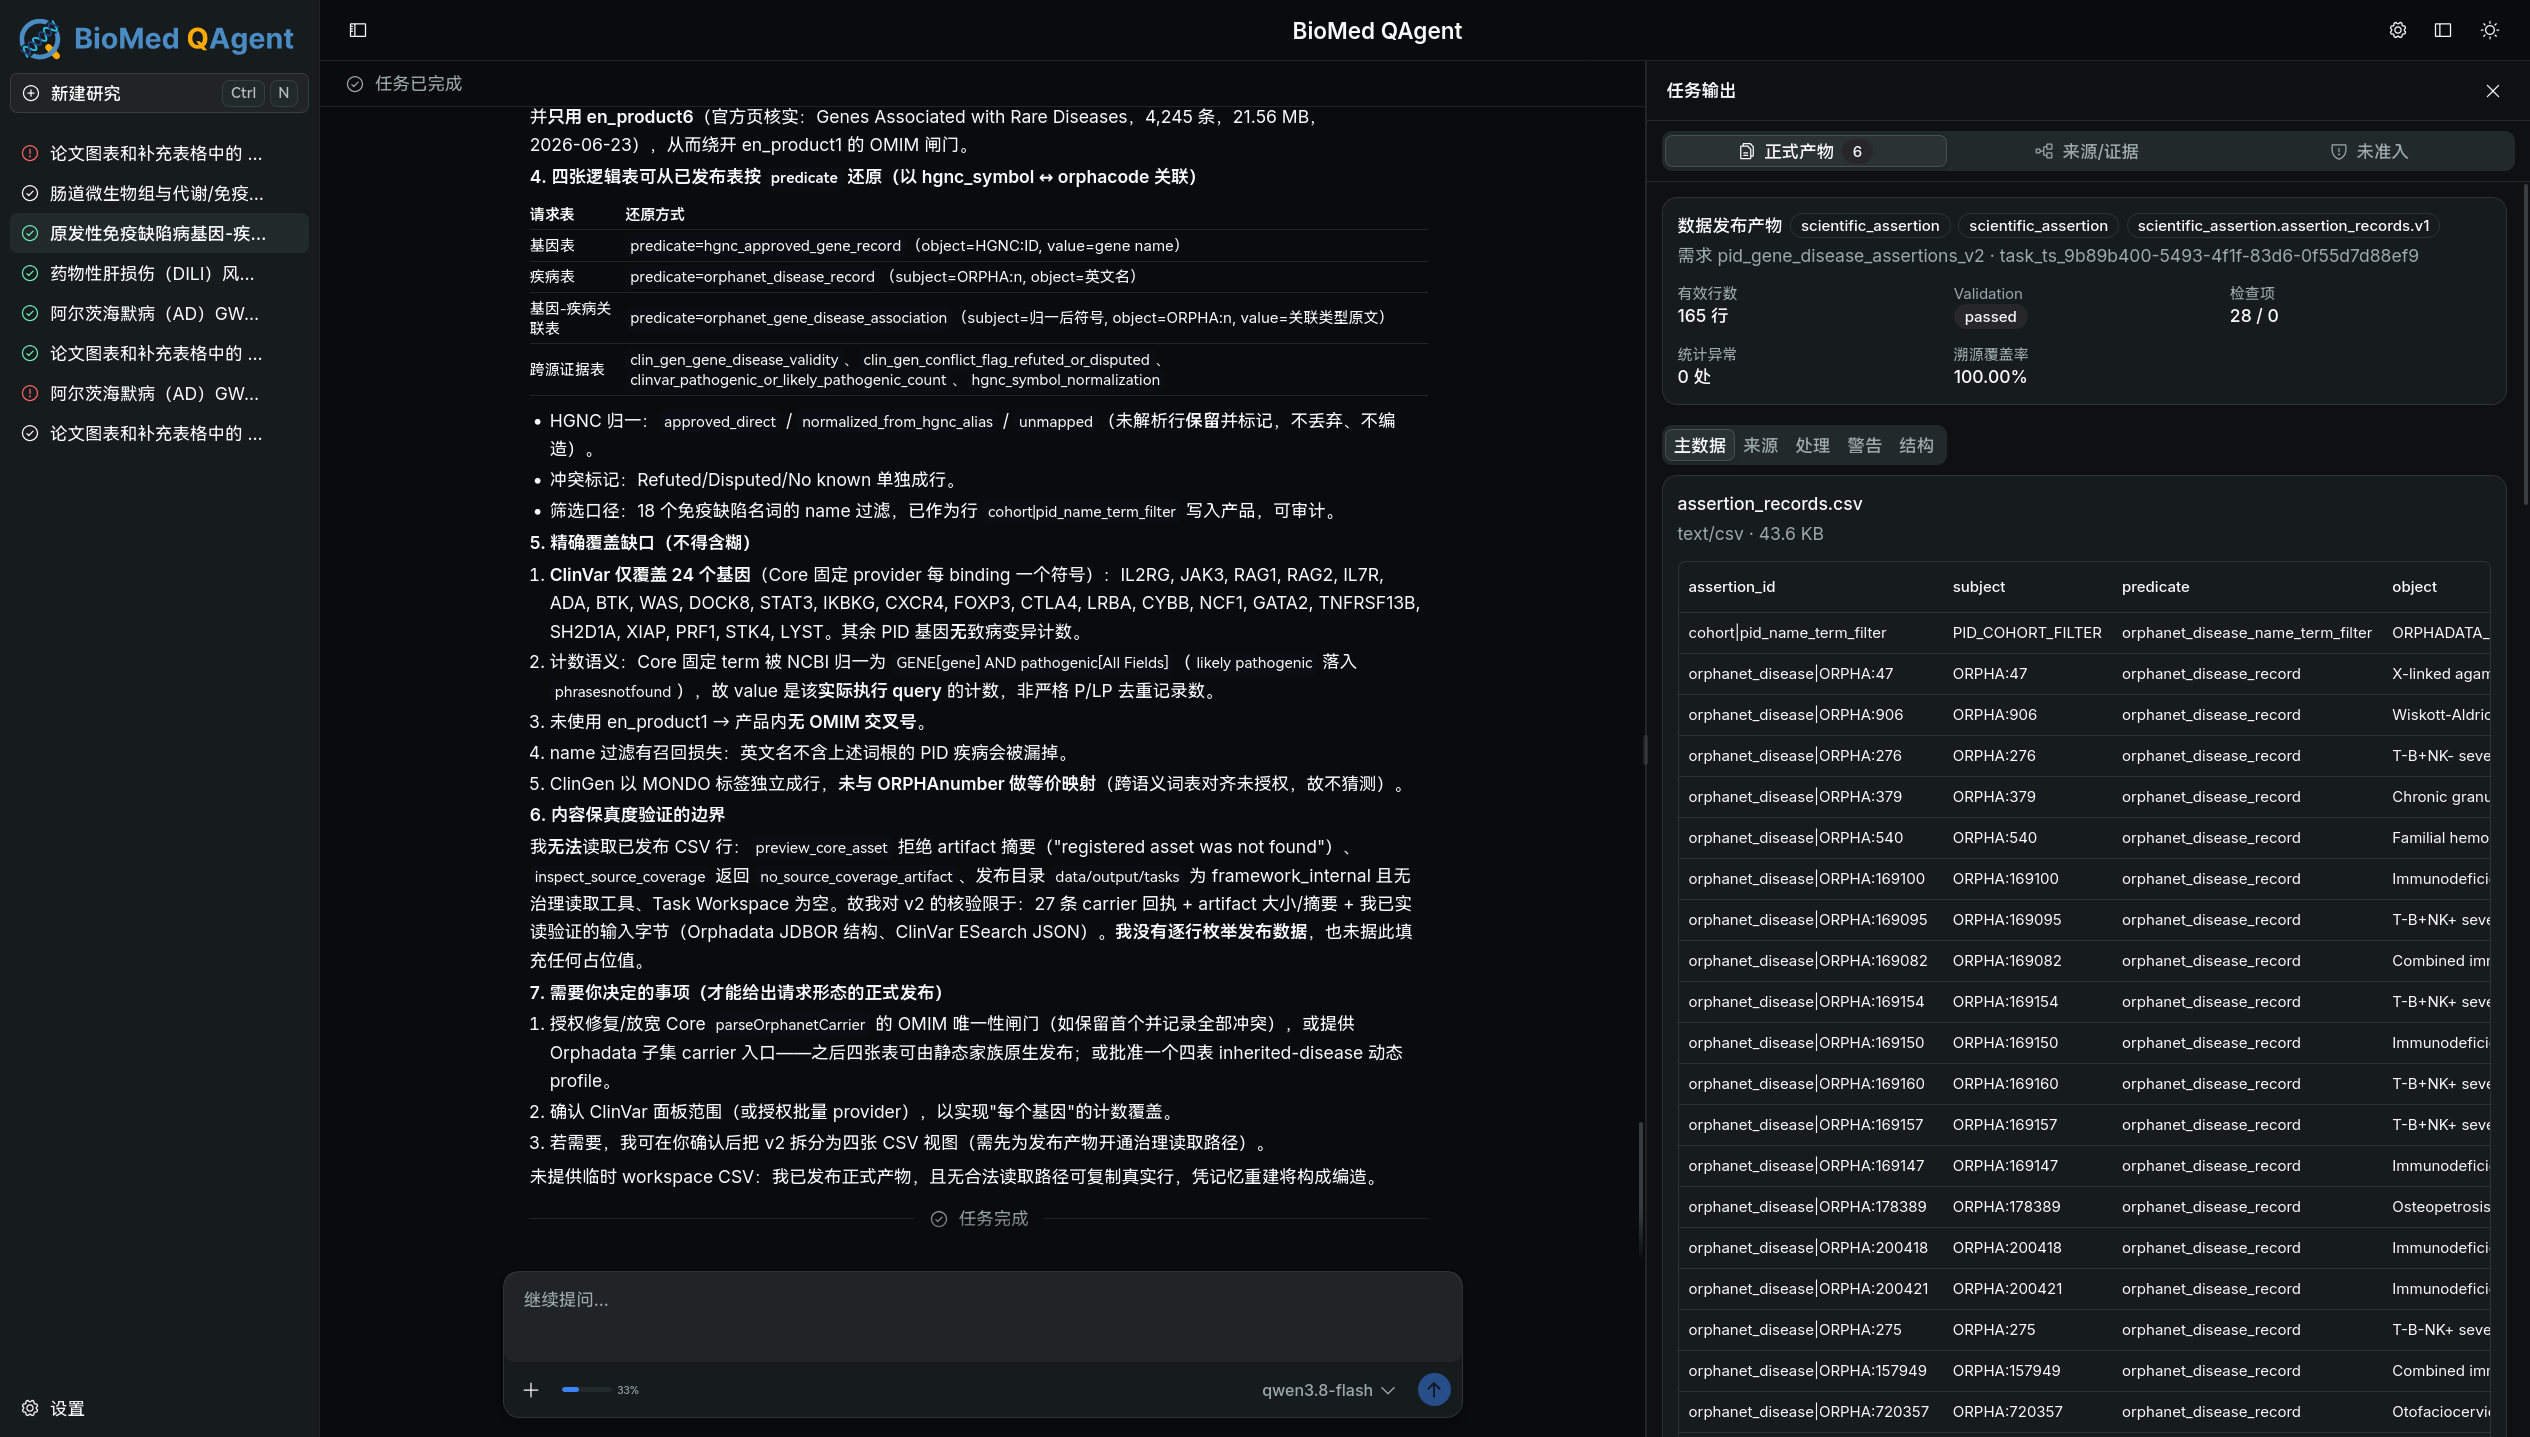
\includegraphics[width=0.90\textwidth]{figures/ui-gold9-artifact-validation.png}
\caption{前端任务工作台。上：来源登记与证据查看；下：发布文件核验与下载。}\label{fig:ui-workbench}
\end{figure}

\begin{figure}[htbp]
\centering
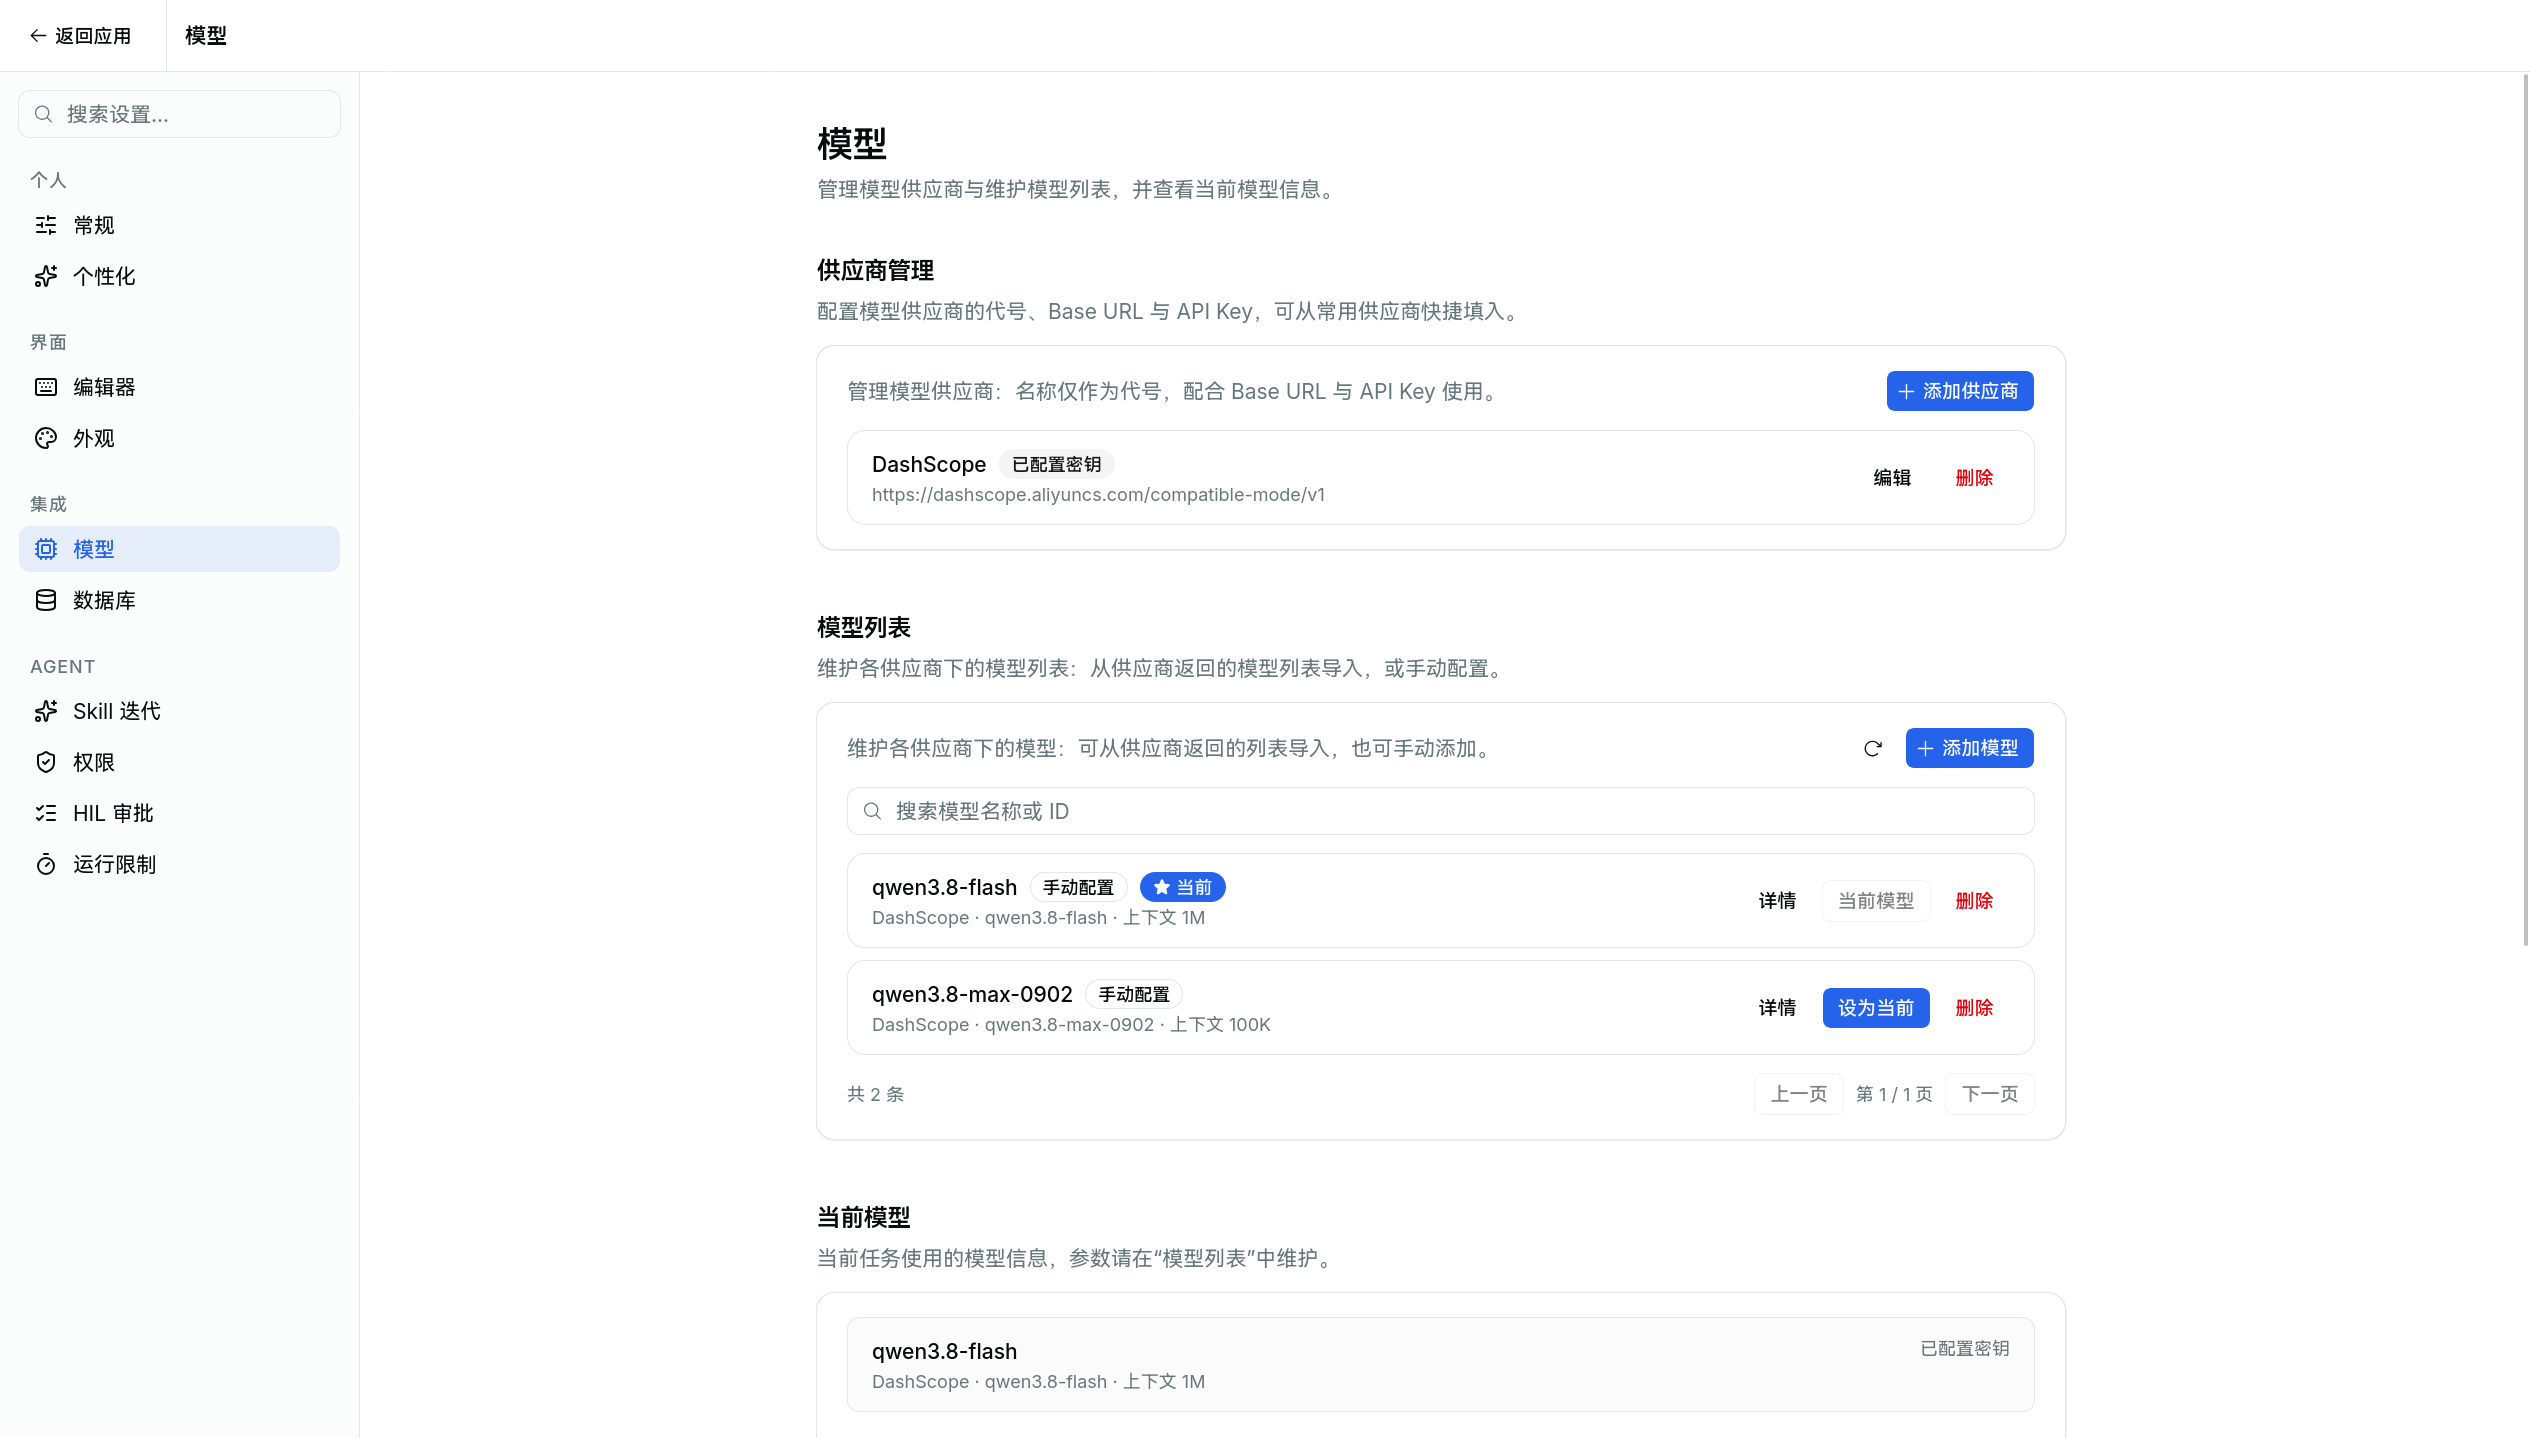
\includegraphics[width=0.88\textwidth]{figures/ui-settings-models.png}
\caption{模型配置界面：可设置模型名称与服务凭据，并单独选择视觉模型。}\label{fig:ui-settings-models}
\end{figure}

\section{三层产物模型}\label{sec:three-layer}

\begin{enumerate}
  \item 工作区暂存结果：搜索下载、模型阅读、探索脚本和临时 CSV 可以辅助任务，但不视为正式交付。
  \item Core 候选结果：来源已经登记，处理步骤有记录，候选表带有表结构、溯源和检查结果；发布条件尚未满足时继续停留在这一层。
  \item 正式发布结果：候选通过发布检查后，系统创建只增不改的发布目录，并记录各文件大小与摘要。读取时再次核验。前端以此标记正式发布成功，同时仍须另行说明需求完成范围。
\end{enumerate}

三层结果分别回答“文件是否存在”“候选是否符合规则”“是否已经正式发布”。工作区允许检索、试算与脚本试错，但仍受文件和工具权限约束；发布检查则决定哪些结果可以正式交付。

当正式采集尚不支持某个来源，而用户已有外部文件时，可将文件上传到任务暂存区，并声明覆盖完整、部分或未知。服务端生成存储标识，计算文件大小和 SHA-256，回执将其标记为不可信参考；下载时重验摘要。该目录与正式发布目录分开，随任务删除。上传回执不能代替来源登记、候选检查或发布许可。

\section{研究需求编译}\label{sec:requirement-compile}

Agent 首先从用户问题中整理出目标实体、数据类型、样本或队列条件、必需字段、期望层级和输出要求。随后，Agent 必须执行一次“路线检查”，确认当前注册表（服务端登记的各项能力清单）支持哪些数据家族、表结构、来源和解析器组合，以及动态路线能够直接绑定哪些数据提供者。

以样例1的“乳腺癌肿瘤与正常组织转录组整合”为例，Agent 需要明确表达表采用探针级还是基因级记录，如何识别样本分组，绑定哪些 GEO 系列与平台注释，以及怎样保存探针—基因对应关系。这些决定写入执行规格，供服务器逐项检查。明确规格并不自动排除遗漏，纳入范围仍须与原始任务核对。

需求编译不是把自由文本简单改写，而是形成数据集执行规格。服务器会交叉校验这份规格：数据家族与表结构是否已注册，行层级与目标实体层级是否一致，每个来源绑定的提供者、解析器和参数是否合法，规范化、合并和校验配置是否在白名单内，输出格式是否受支持，以及多表输入的角色关系是否闭合。任一项不通过，系统都会阻断执行或要求修正。

路线指执行数据构建的固定路径：静态路线使用注册表中现成的数据家族与解析器；动态路线允许Agent为未注册的多表结构临时申请一条受控执行路径。如果注册表能够精确表达需求，Agent 采用静态路线。如果静态结构不匹配，但所有输入都能由Core 的提供者获取（或已经是任务拥有的来源资产），Agent 可以采用动态路线。两条路线都无法闭合时，系统只交付明确标记为暂存的结果，并列出缺失的正式能力，不将其伪装成正式发布。

\section{候选来源发现}\label{sec:source-discovery}

Agent 可以组合文献 API、专业数据库、补充材料归档和网页搜索。文献查询采用主题词与同义词，数据库查询使用实体标识与字段，网页搜索补充预置通道之外的入口。检索结果包括数据集编号、论文、附件、下载地址及其字段和范围。不同通道返回的信息可以互查，但同一来源多次出现不等于增加了独立证据。

来源发现的自主性在样例8 的一次重跑中有直观体现。这次任务（药物性肝损伤）中，官方DILIrank 文件持续返回404，Agent 没有停留在反复重试上，而是经受控浏览器访问搜索引擎结果页，从命中记录中找到LiverTox 官方通道，先后完成16 次页面读取与13 次取证下载，并对5 组openFDA 不良事件查询作交叉核对，全程没有请求权限，也没有人工提示。与之配套的是止损规则：浏览器通道对同一主机的连接性失败连续达到阈值即短路，返回结构化的“无数据”信号。早期运行曾观测到对同一失效地址连续555 次顺序枚举的空转，这条规则就是为了阻断这类行为。

Core 按规格中的来源绑定记录检索计划与采集结果。记录包括查询参数、采集回执、解析与保留行数、拒绝及排除原因、请求上限，以及成功、失败、尚未尝试的来源数量。Agent 可以据此调整查询或补充来源，避免将失败来源从最终说明中省略。

来源覆盖统计只回答“计划中的来源处理了多少”。未纳入计划的数据库、未发现的附件不在分母内，因此该比例不能代表问题子领域已经查全。计划外遗漏需要用独立整理的参考来源集合核对。预置通道之外的材料可以经声明式 HTTP 接入、浏览器取证或任务上传进入系统；正式采用前仍需登记来源并接受检查。

\section{Agent 的自主决策面}\label{sec:agent-autonomy}

Agent 与Core 的分工可以概括为：Agent 负责开放式的研究决策，设计数据产品；Core 负责按确定性规则实现设计，并验证其是否可以交付。Agent 的自主性体现在数据产品生产的各个决策点上（表~\ref{tab:decision-inventory}）。Core 约束的是这些决策进入正式数据的通道，而不是决策本身。Core 拒绝的是执行期的任意DAG 编排：Agent 不能提交自定义的处理节点链、合并函数或发布路径。数据模型层面的多表拓扑设计（表、主外键与角色映射）属于Agent 的决策面，二者分属执行编排与产品结构两个层面。

\begin{table}[htbp]
\centering
\caption{Agent 的自主决策清单}\label{tab:decision-inventory}
\begin{tabularx}{\linewidth}{>{\hsize=0.40000\hsize}L>{\hsize=1.30000\hsize}L>{\hsize=1.30000\hsize}L}
\toprule
\textbf{决策点} & \textbf{Agent 自主决定} & \textbf{Core 的约束} \\
\midrule
检索与来源 & 组合查询、比较候选、决定采集对象和顺序 & 正式输入需由注册提供者获取或登记为任务来源资产 \\
执行路线 & 选择静态路线，或提出表、主外键、角色映射与来源绑定 & 规格先检查，候选文件逐件重新计算摘要 \\
规格迭代 & 依据错误说明修正表结构与参数 & 逐字段返回拒绝原因；不通过则不执行 \\
质量与修正 & 决定补源、修改规格、重新提交或说明未完成部分 & 新发布保留旧文件；已触发的审批按规则处理 \\
数据值 & 提出字段映射、单位换算和抽取候选 & 候选必须经过准入、完整性检查、产品评估与发布检查；检查不等于自动证明数值正确 \\
\bottomrule
\end{tabularx}
\end{table}

\section{LLM 使用方法与上下文工程}

本节说明Dataset Core 之外的Agent 侧如何使用LLM 以及如何组织上下文，对应\ref{sec:contributions} 节的贡献一。证据上下文控制（\ref{subsec:evidence-context} 节）与第第\ref{ch:dataset-core}章的确定性校验上限和人工确认机制直接衔接。

\subsection{完成规则与运行状态注入}\label{subsec:completion-contract}

系统提示要求 Agent 区分正式发布和任务完成。数据生产请求只有取得本次运行的正式发布物及其清单，才可报告“发布成功”；仅有临时 CSV 或自写文件清单不满足这一条件。报告还须说明已交付与未交付的任务条目，不能因某个较小规格执行成功而宣称原任务全部完成。

完成判定也有提示词之外的支撑。运行时每回合都会注入一条由事件流压缩而成的运行状态，内容包括当前阶段（规划/执行/等待工具/收尾）、工具调用的成败计数、是否已存在不可变发布物，以及下一步建议，例如“仍有N 个工具在执行，不要假定其结果”，或“最近一次失败为某工具，仅在可重试或换用独立来源时重试”。这样，完成与否以数据产品的实际状态为依据，而不是以模型对自身行为的记忆为依据。

\subsection{行为约束：从实测失败模式到提示规则}\label{subsec:behavior-rules}

系统提示词中的行为约束来自对模型失败模式的实际观察。开发期在同一个表达组学案例（乳腺癌GEO 表达整合）上的提示词迭代记录显示，轻量模型在无人工干预的长流程中反复出现三类行为偏差。其一，时限幻觉：某次运行在240 回合的预算仅使用35 次模型调用时，以“由于时间限制和复杂性”宣布放弃并等待用户指示，而系统从未设置任何时限。其二，重复失败：对同一数据集以同一套参数连续失败七次，仍不改变策略或换用其他来源。其三，发布后反复自检：正式发布完成后，模型反复重读已经验证过的回执，一次运行中这部分重复验证消耗了全部计费token 的79\%。

系统提示词针对这三类行为逐条写入了约束：声明系统不以未经配置的总时限为放弃理由，回合与上下文预算只是防止失控的上限，不允许以时间限制为理由放弃任务；同一错误重复出现时，立即停止同形态重试，改为查清被拒绝的具体原因，或换用真正独立的来源；每件发布产物只验证一次，验证后记录结论并转入最终报告。决策方式也作了相应调整：不确定某个工具或检查如何运行时，直接阅读它的实现源码，以代码为准判断“接受什么输入”，而不是凭记忆反复试错。

在一组前后对照的迭代中，同一案例、同一模型、同一任务的工具调用从60 次降到36 次，计费token 从5.71M 降到3.73M，工具错误从7 次以上降到2 次。迭代中也识别出一些值得保留的行为模式，如单平台同粒度设计优先、拒绝跨研究拼接行、发现映射未经验证时主动修订而不是宣称完成；这些模式随后写入流程技能，成为后续运行的默认规则。该迭代发生在第五章评测之前，用于校准提示词，不计入评测结果。

\subsection{路由预检与声明式工具结构描述}

\mbox{BioMed QAgent} 向大模型公开当前真实能力及相关参数。静态路线要求精确匹配注册表中的数据家族、表结构与来源能力清单；动态路线只接受预检报告确认可以绑定的输入。工具参数的结构描述严格约束字段类型、枚举、对象结构和必要参数，服务器端还会进行交叉验证。

上下文工程的重点不是把所有代码放进提示词，而是提供模型决策所需的最小必要信息。这些信息包括：当前任务与研究目标，可用工具及其严格输入结构，注册表返回的数据家族、表结构和提供者能力，来源搜索结果与失败回执，校验问题、人工确认选项及证据摘要，以及当前发布物或阻塞状态。这样可以把“模型知道什么”绑定到运行时的实际能力，减少提示词与代码版本之间的漂移。

\subsection{技能体系与专用工具}\label{subsec:skills}

专用能力按数据库访问、载体取证和任务流程三类组织。技能描述入口、查询方式、字段含义和使用步骤，工具执行具体操作；其结果是否可以正式采用，仍由 Core 检查。

其一，数据库类技能14 项：PubMed、GEO、GDC、Xena、UniProt、PDB、PubChem、ChEMBL、ClinVar、GWAS Catalog、dbSNP、MGnify、openFDA、Reactome——每项封装对应入口的查询、分页与来源特有字段，Agent 不必为每个站点编写脚本。

其二，载体与取证技能：包括浏览器导航与页面取证、PDF 表格提取、图表视觉提取（qwen3.8-flash）、文献理解、网页视觉取证、搜索发现和本地缓存复用。

流程类技能包括数据集构建引导、研究数据指引和分析。构建引导要求先检查执行路线，再编写与校验规格，最后核对正式发布物；研究数据指引说明如何选择来源、清洗数据并记录未查来源。分析技能可以辅助查看结果，但不取代正式数据发布，也不代表系统已经验证科学结论。

在已有访问方式和解析器能够处理目标数据时，可以通过声明式配置扩展来源。新协议或新格式仍需补充相应代码。工具返回结构化结果与错误，供 Agent 调整查询或说明缺口；新增技能不会绕过网络权限、来源登记与发布检查。

\subsection{证据上下文与不确定性控制}\label{subsec:evidence-context}

模型不应仅看到最终值，还应看到该值的来源类别、定位信息、解析层级和置信度。对于非确定性抽取，系统记录该值的置信类别、给出该类别的理由、执行抽取的模型与其提示版本、以及是否经过人工复核，并在Core 中设置可信度上限。

模型提出字段映射、单位修正或抽取值时，应同时说明依据。正式采纳取决于注册规则、候选检查和必要的人工决定。证据类型分级用于安排检查，不应写成经过统计校准的正确概率。

